\chapter{Methodology}\label{chap:method}

\section*{}
In this chapter all the process that led to achieving the main goal of the thesis, predict the deformations caused by BCS is described in detail.
In order to plan such process, the study on breast cancer and how to represent the Breast as a 3D model will be used, as well as the developed tool described in chapter \ref{chap:tool}.

The applied methodology is divided in 3 fundamental parts: a dataset preparation to feed the following steps, the application of Machine Learning in order to predict the deformations on the patient's breasts caused by the BCCT, and the validation of the obtained results through several metrics. Those three steps are represented on Figure \ref{fig:method_FC} and are detail through the several sections on this chapter.

\begin{figure}[!h]
\begin{center}
    \leavevmode
    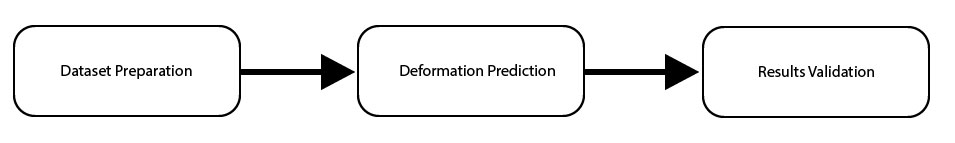
\includegraphics[width=0.85\textwidth]{method_FC}
    \caption[Flowchart of the applied methodology]{Flowchart of the applied methodology}
    \label{fig:method_FC}
  \end{center}
\end{figure}

\section{Dataset Preparation}\label{sec:dataset_prep}

In order to further apply machine learning techniques to predict the deformations on the patient's breast, a semi-synthetic dataset was prepared. Despite of existing a few datasets with 3D models of the breast, they are constructed based on a generic shape of the breast with some deformations applied to it. Although the great amount of studied deformations, they are still unable to represent the variability and diversity that may be found in a semi-synthetic dataset. This created semi-synthetic dataset contains 3D breast models representing the patient's breast before and after the surgery. The pre-surgical models in the dataset are based on the real data obtained though MRI data of a few patients. The pos-surgical models are generated by taking as parameters the hypothetical tumor's location and volume and the breast's density. Considering different parametrization, each pre-surgery model of the dataset defer from other regarding the following features:
\begin{itemize}
\item breast's density,
\item breast's volume,
\item breast's laterality,
\item tumor's position
\item tumor's volume.
\end{itemize} 
The pos-surgery 3D models of the breast are obtained though a biomechanical simulation of the wound healing based on the pre-surgical models generated through the patients' MRI data. The BCS planning tool described in chapter \ref{chap:tool} was used to generate the hyphothetical tumor's location and volume. The pre-surgery models will be used to simulate the pos-surgery models alongside with the hyphotetical tumor's location and size through a biomechanical healing simulator described in \cite{Vavourakis2016}. Figure \ref{fig:data_WF} illustrates the workflow of the steps pursued for preparing the dataset.

\begin{figure}[!h]
\begin{center}
    \leavevmode
    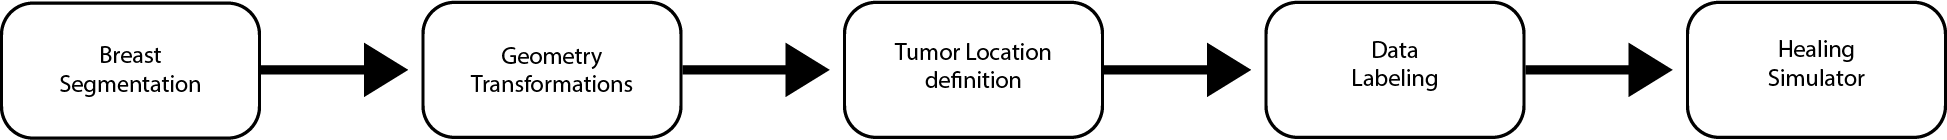
\includegraphics[width=1.0\textwidth]{data_WF}
    \caption[Flowchart for the dataset generation]{Flowchart for the dataset generation}
    \label{fig:data_WF}
  \end{center}
\end{figure}

Initially, it is necessary to segment the breast outline from background of the MRI data for each initial real patient. Further, a 3D model is reconstructed from the segmented data. However, since the MRI is taken as the patient is lied in prone position, it is necessary to apply a geometry deformation to represent the breast in a supine configuration. With the proper geometry, the tumor must be defined in the specific breast, that therefore will be labelled according with the healthy and damaged portions of the breast. At last, the wound healing simulation will be performed in order to generate the pos-surgical model of the breast.


\subsection{Breast segmentation}

As described before, the pre-surgical 3D models of the patients' breast were constructed based on MRI data segmentation. The breast segmentation is performed by annotating both the breast and the pectoral muscle. The annotation included both left and right breast with the respective nipple and had as lateral boundaries the left and right latissimus dorsi. The pectoral muscle included both the right and left major and minor pectoral muscles. Figure \ref{fig:latissimus} depicts the anatomical structure mentioned during segmentation. The result of a patient annotation used to generate the breast's point cloud is shown in Figure \ref{fig:pre_model_annotation}.

\begin{figure}[!htb]
\begin{center}
    \leavevmode
    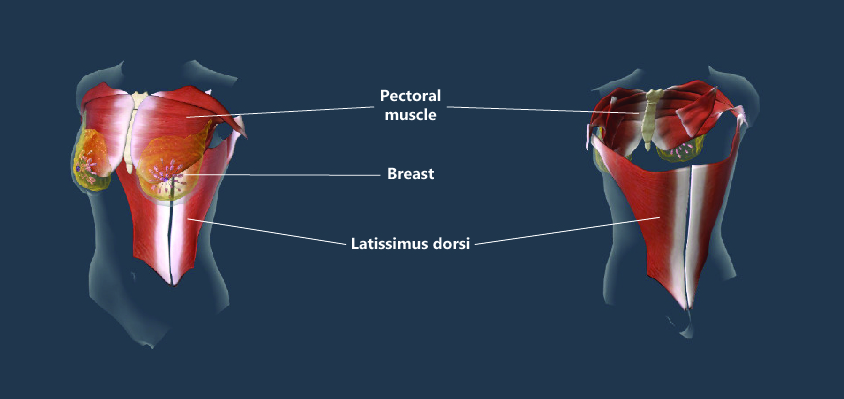
\includegraphics[width=0.85\textwidth]{latissimus}
    \caption[Representation of the Breast, Pectoral muscle and Latissimus Dorsi]{Representation of the Breast, Pectoral muscle and Latissimus Dorsi}
    \label{fig:latissimus}
  \end{center}
\end{figure}

\begin{figure}[!htb]
\begin{center}
    \leavevmode
    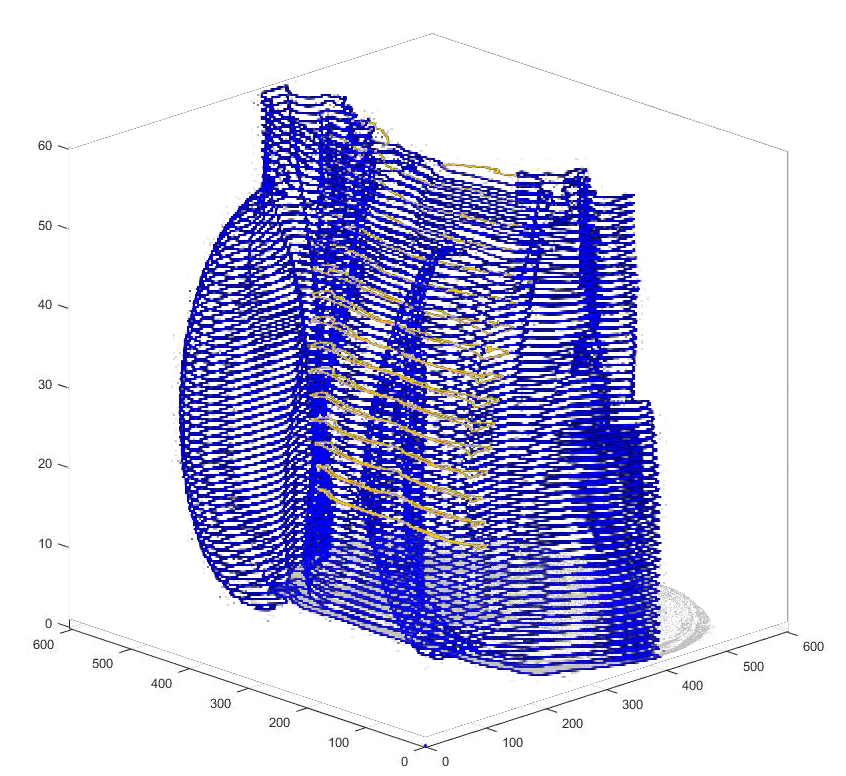
\includegraphics[width=0.45\textwidth]{pre-model}
    \caption[Breast Segmentation result]{Breast Segmentation result for one of the patients}
    \label{fig:pre_model_annotation}
  \end{center}
\end{figure}

All the annotations were made using MARge Tool to appear in \cite{marge}, whose interface is displayed in Figure \ref{fig:marge}.

\begin{figure}[!h]
\begin{center}
    \leavevmode
    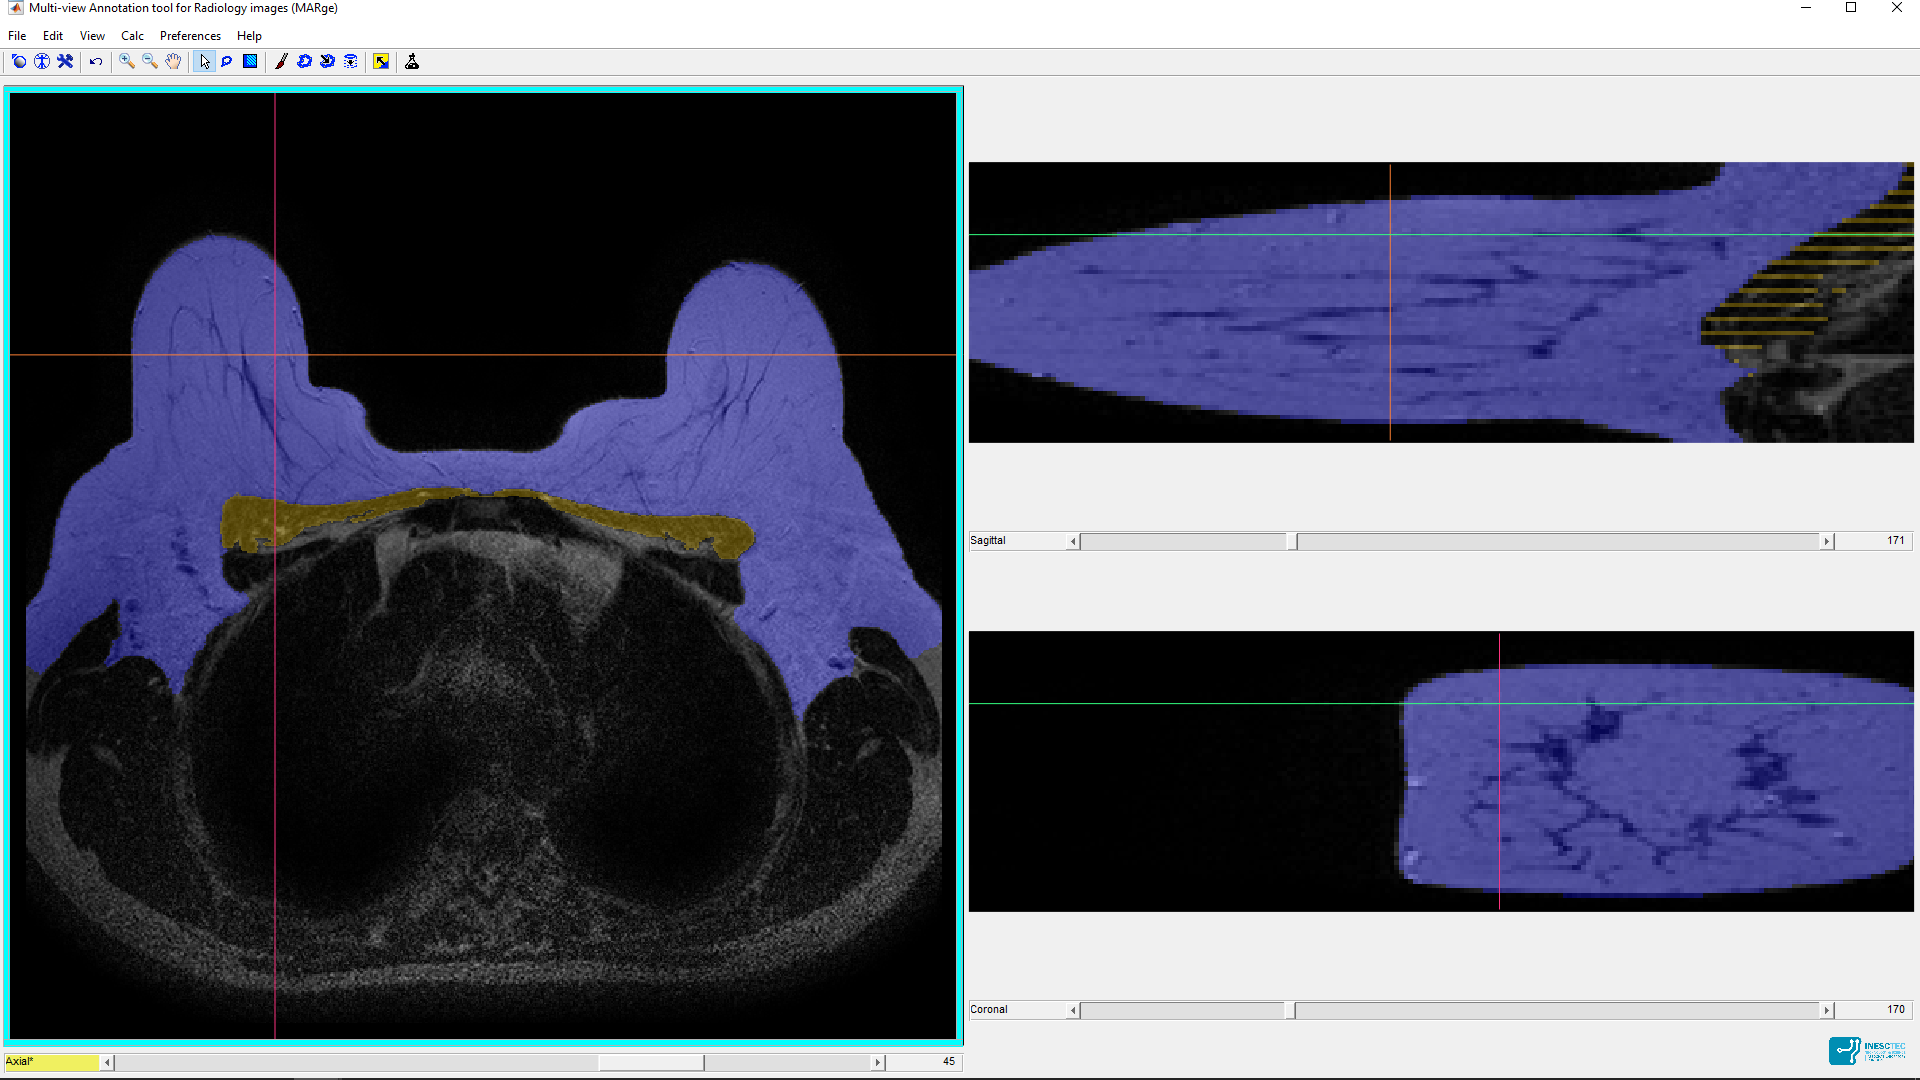
\includegraphics[width=0.70\textwidth]{marge}
    \caption[Interface of MARge tool used for the breast segmentation]{Interface of MARge tool used for the breast segmentation}
    \label{fig:marge}
  \end{center}
\end{figure}

\subsection{Geometry Transformations}\label{subsec:geometry_transf}

After the segmentation of the patient's MRI data, the meshes regarding the pre-surgery models were generated. While the MRI acquisition is done in prone, the tumor definition and posteriorly the surgical simulation need the model in a supine geometry. The transformation between the prone and the supine geometries were performed recurring to a Bio-mechanical simulator described in \cite{Vavourakis2016}. In order to perform these transformation a virtually state known as unloaded geometry was required. In the unloaded geometry, the force of gravity and other tension or stress forces are ignored \cite{Iben2016}. The same biomechanical simulator is used to generate the pre-surgical model in a upright geometry (from the unloaded model) that will be further used. The aesthetic evaluation of the breast is performed in a upright position. The impact of changing the direction of gravity vector to a breast model is depicted in Figure \ref{fig:breast_geometry}.

\begin{figure}[!htb]
\centering
\scalebox{0.73}{%
\begin{tabular}{cc}
\subfloat[3D view of Prone geometry]{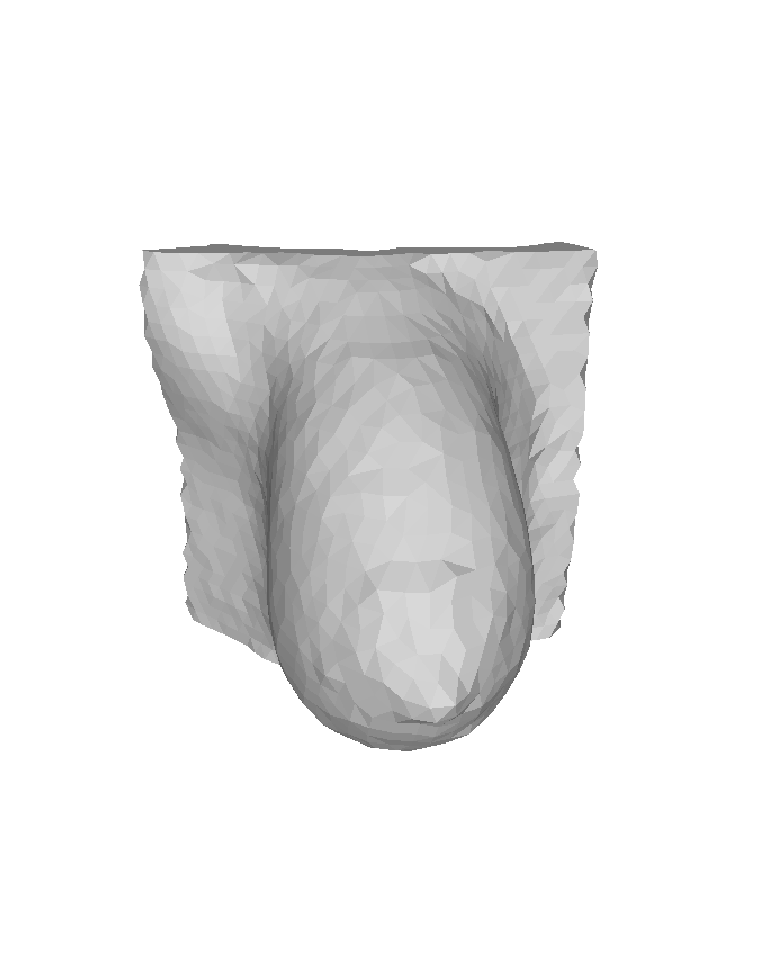
\includegraphics[width = 2in]{prone}\label{fig:prone}} &
\subfloat[Lateral view of Prone geometry]{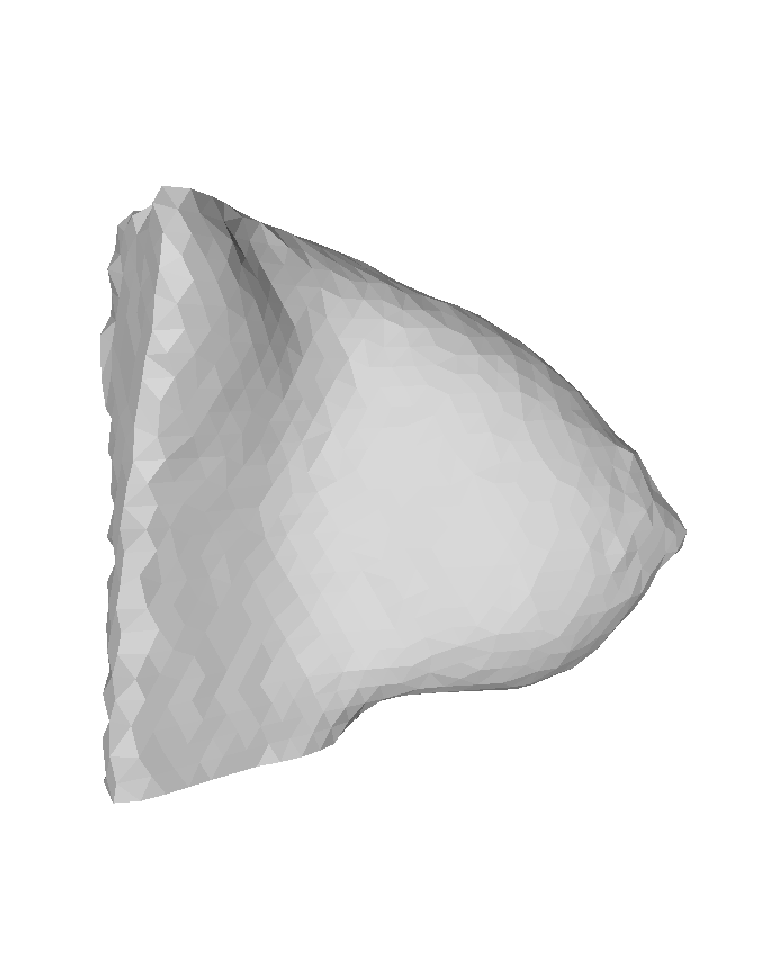
\includegraphics[width = 2in]{prone_l}\label{fig:prone_l}}\\
\subfloat[3D view of Unloaded geometry]{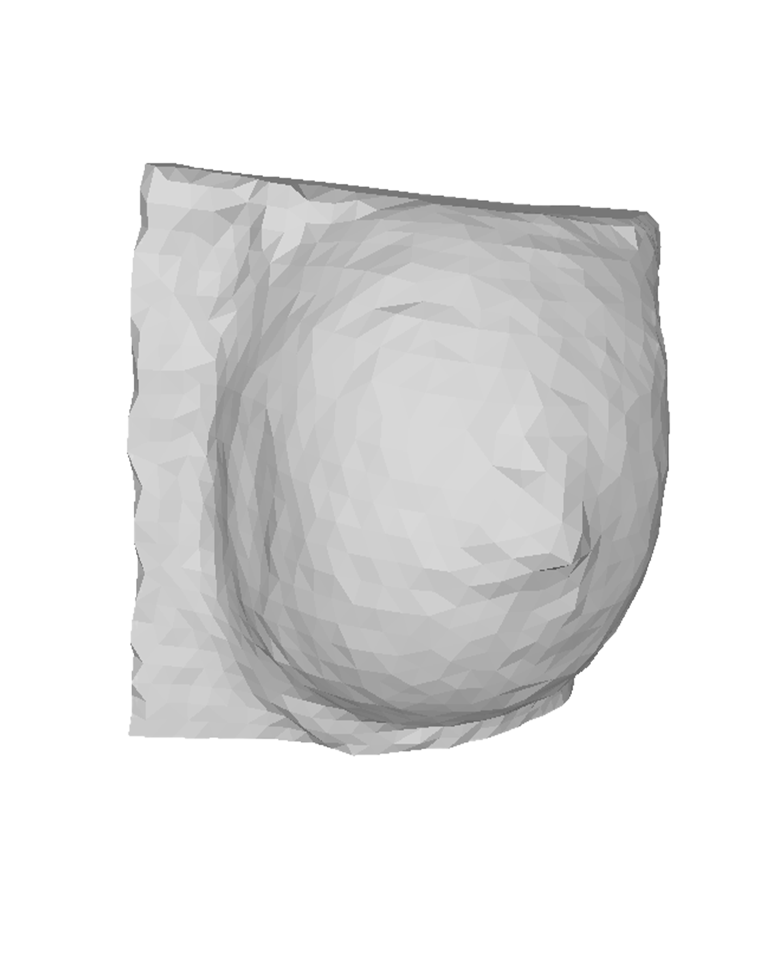
\includegraphics[width = 2in]{unloaded}\label{fig:unloaded}} &
\subfloat[Lateral view of Unloaded geometry]{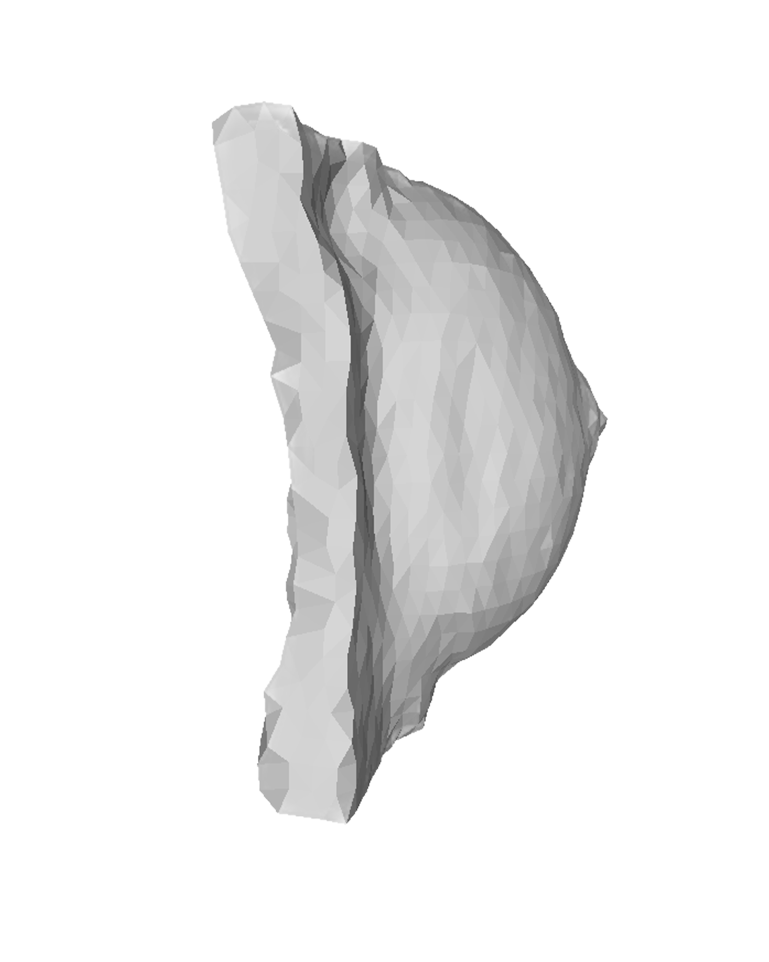
\includegraphics[width = 2in]{unloaded_l}\label{fig:unloaded_l}}\\
\subfloat[3D view of Supine geometry]{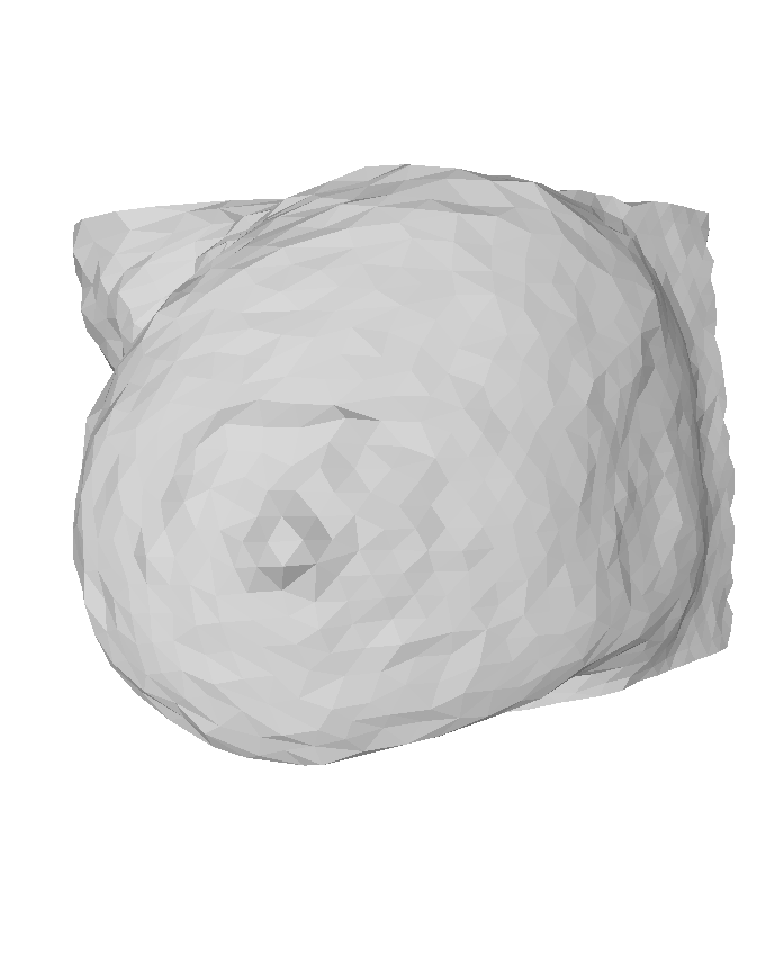
\includegraphics[width = 2in]{supine}\label{fig:supine}} &
\subfloat[Lateral view of Supine geometry]{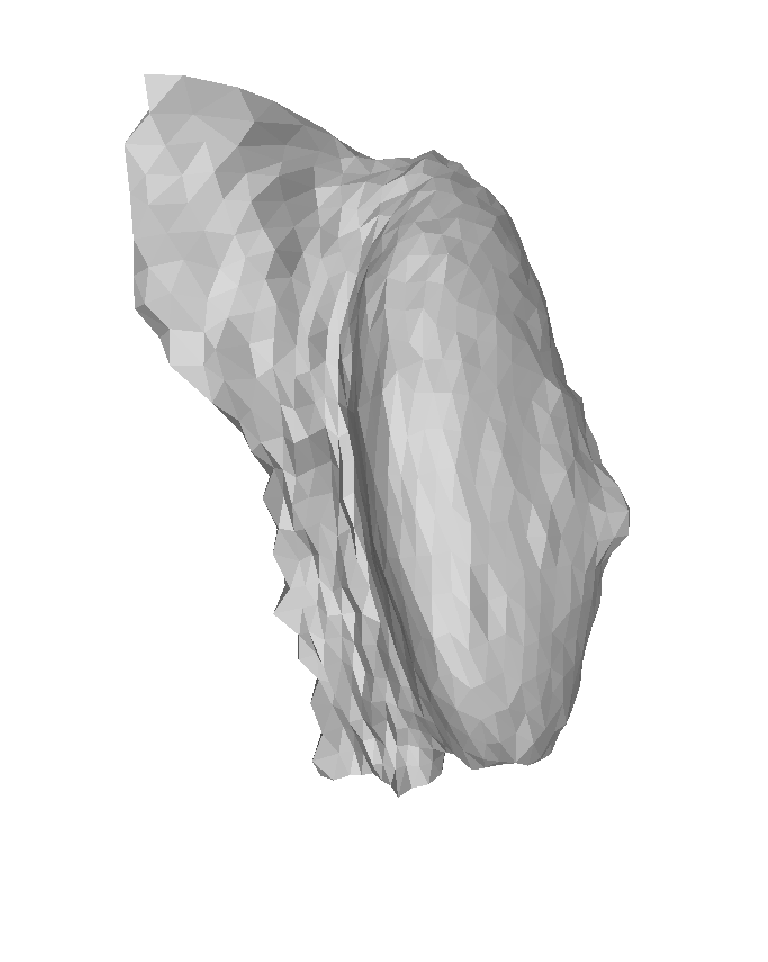
\includegraphics[width = 2in]{supine_l}\label{fig:supine_l}}\\
\subfloat[3D view of Upright geometry]{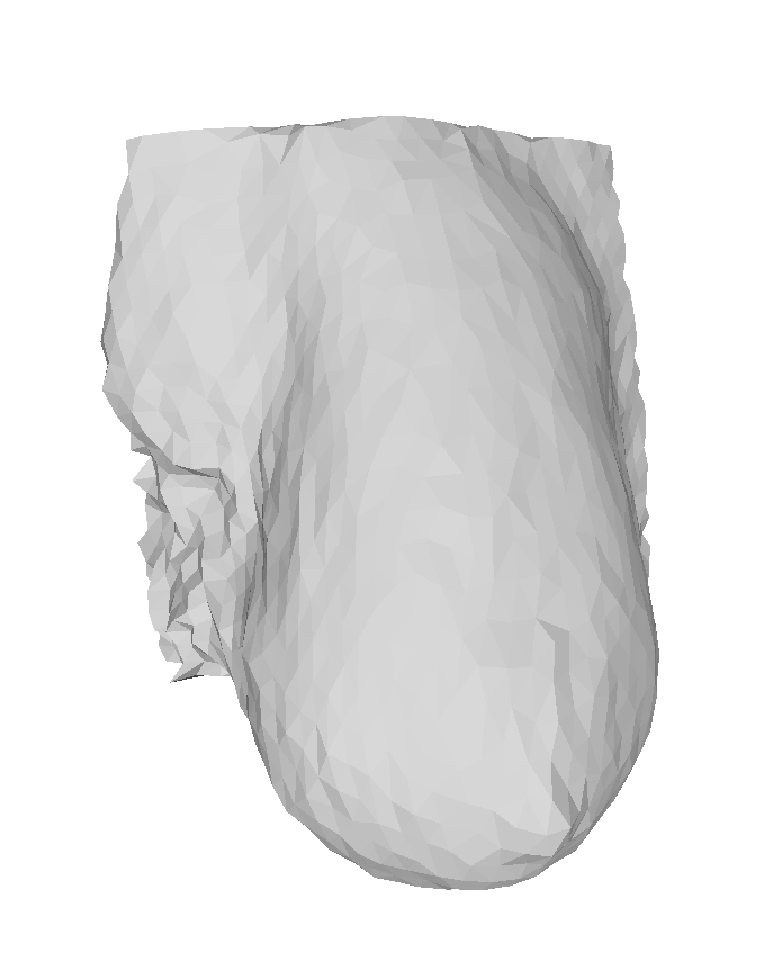
\includegraphics[width = 2in]{upright}\label{fig:upright}} &
\subfloat[Lateral view of Upright geometry]{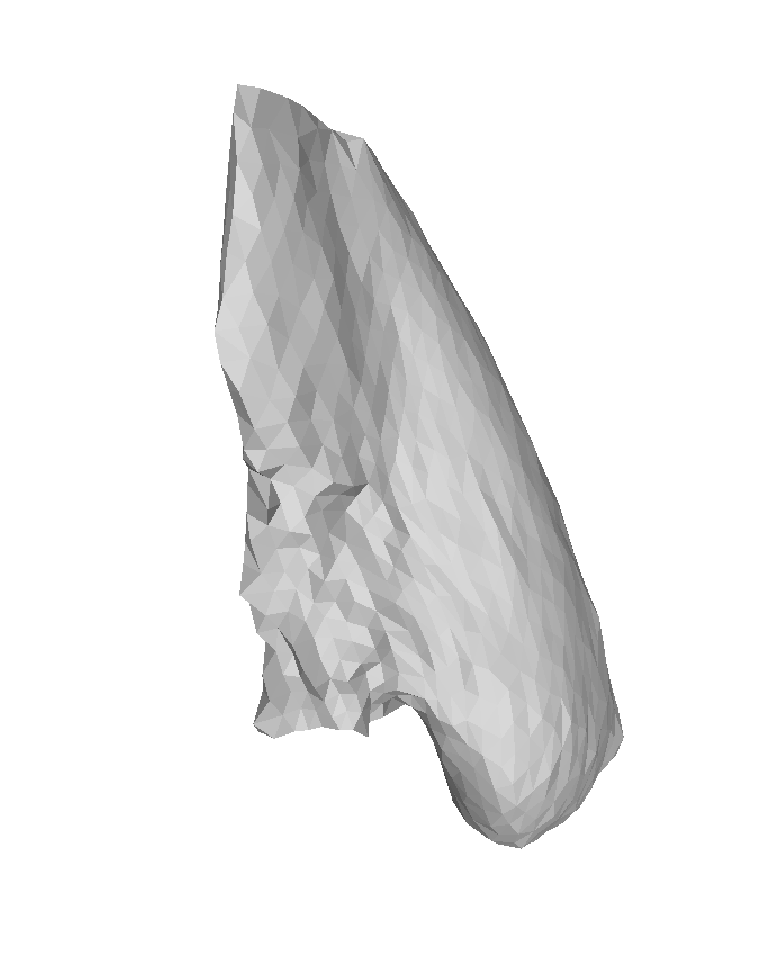
\includegraphics[width= 2in]{upright_l}\label{fig:upright_l}}
\end{tabular}
}
\caption[3D breast geometry transformations]{3D breast geometry transformations}
\label{fig:breast_geometry}
\end{figure}


\subsection{Tumor's location definition}\label{subsection:tumor_location}

The tumor definition is done recurring to the tool described in chapter \ref{chap:tool}. The tool will take as input the pre-surgery model in a supine geometry and query the user for a tumor position. By selecting the tumor's position, it will be categorized according to one of the four quadrants of the breast also defined as regions, as shown in Figure \ref{fig:regions}:
\begin{itemize}
\item R1 - Upper-Outer quadrant of the breast;
\item R2 - Upper-Inner quadrant of the breast;
\item R3 - Lower-Outer quadrant of the breast;
\item R4 - Lower-Inner quadrant of the breast.
\end{itemize}

\begin{figure}[!htb]
\begin{center}
    \leavevmode
    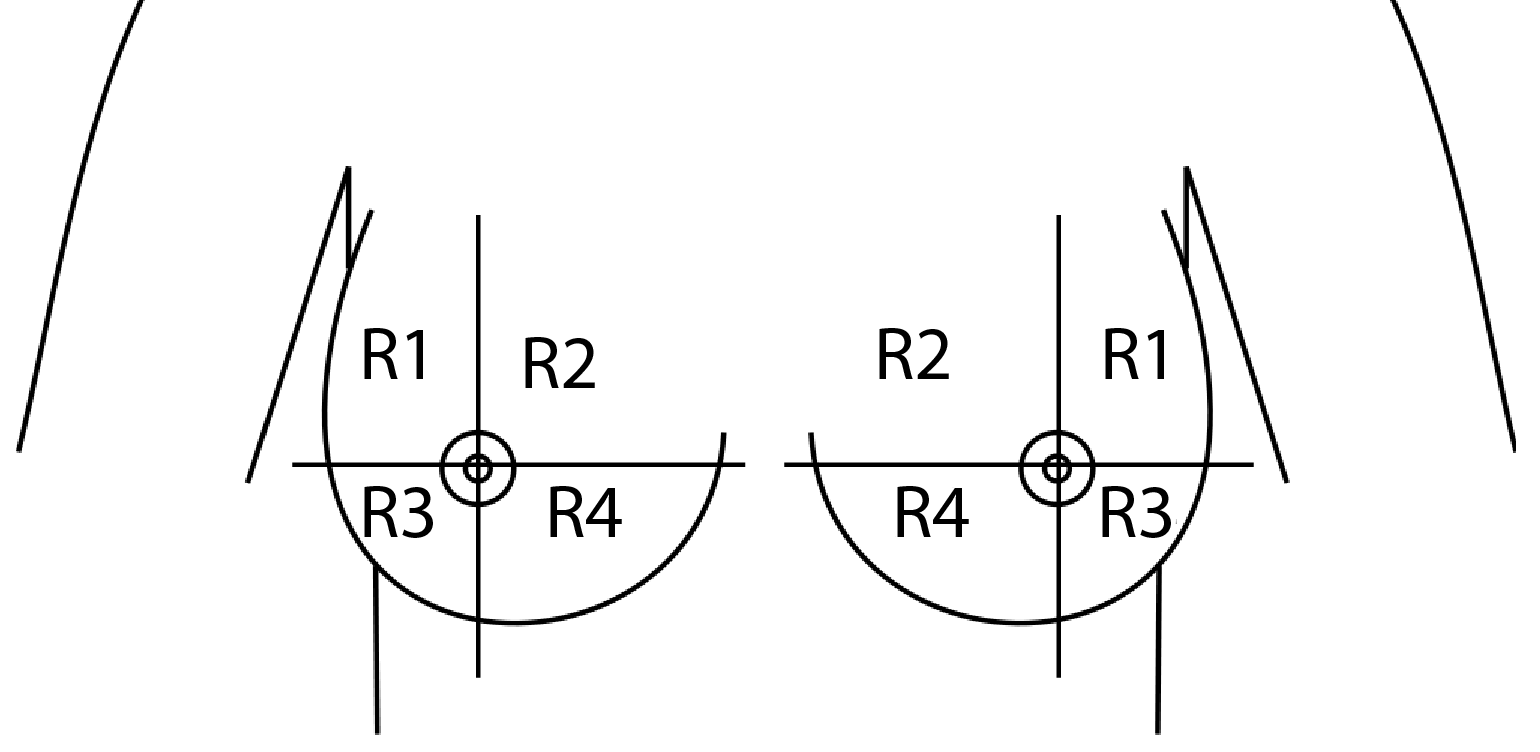
\includegraphics[width=0.55\textwidth]{quadrants}
    \caption[Breast quadrants used for tumor location]{Breast quadrants used for tumor location}
    \label{fig:regions}
  \end{center}
\end{figure}


Thereafter a mesh containing the tumor in the defined region with one of the predefined sizes as follows will be generated:

\begin{itemize}
\item A small size - corresponding to 5\% of the total breast's volume;
\item A medium size - corresponding to 7.5\% of the total breast's volume;
\item And a large size - corresponding to 10\% of the total breast's volume.
\end{itemize}


The percentages used as default for the tumor's size were obtained through discussion with physicians to understand the approximate size of the tumor in different stages of cancer detection.

The produced tumor will be represented by a cylinder centred on the chosen position for the tumor and perpendicular to the chest wall going from the pectoral muscle to the skin contour of the breast. The cylinder's radius is calculated based on the tumor size. All the process is visually supervisioned and the results for the tumor need to be accepted by the user. As result a mesh with exact shape of the one used as input will be generated and posteriorly labelled to be used on the surgical simulation. The labelling process is explained in section \ref{subsection:labelling}.


\subsection{Data Labelling}\label{subsection:labelling}

The labeling is done based on the mesh and what each point and element represents. There will be different labels for surface and volumetric information. The assigned labels indicate the following boundaries of the mesh: front, pectoral muscle or back, left and right or top and bottom. However, the lateral and top and bottom sides of the model are not deformed by the biomechanical neither the wound healing models. The volumetric information is labeled according with the material that it is represented and if it is considered healthy on the case of the breast or damaged on the case of the tumor. While the approach of \cite{Vavourakis2016} divides the volumetric elements in fat and glandular tissue, we assume the same type of material for the all breast. This material's properties are set in order to represent the breast's density according with its ACR (from I to IV). According to \cite{Engineering2008}, using two different material to represent both the fat and glandular tissues, instead of using only one material to represent the whole breast do not significantly affect the results.

In order to visualize the models, a format file exchange is required. While this tool and the one presented on the next subsection require files in a \textit{msh} format, to visualize the models the files must be parsed to a \textit{ply} format. This is done through a parser developed in c++.

After defining damaged or healthy labels, the model will be transformed from supine into the unloaded geometry in order to serve as input on the next step, the surgical simulator, as described in subsection \ref{subsec:geometry_transf}. All the information that is required on this transformations and for the wound healing application (including tumor location and volume and breast's density) is automatically generated by the tool presented in chapter \ref{chap:tool}.


\subsection{Wound healing simulation}\label{subsection:wound_healing_simulation}

The wound healing simulation, where the pos-surgical models are generated, is performed through the application of FEM and Multiscale Mechano-Biological expressions \cite{Vavourakis2016}. 
This will provide what would be the pos-surgical model of the patient's breast roughly 6 months (180 days) after the surgery, taking into consideration the patients breast density, the tumor's location and size that were artificially introduced before. Figure \ref{fig:WHS} demonstrates the breast generated by the wound healing simulation in an upright geometry.

\begin{figure}[H]
    \centering
    \subfloat[Frontal view]{{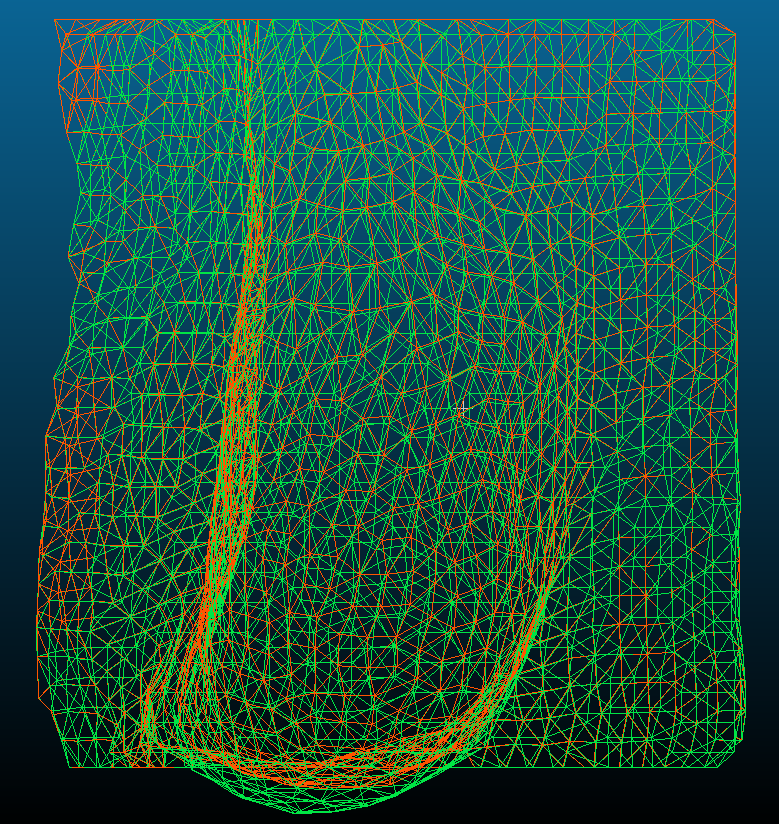
\includegraphics[width=4.5cm, height=4.5cm]{WH_example_frt} }}
    \qquad
    \subfloat[Lateral view]{{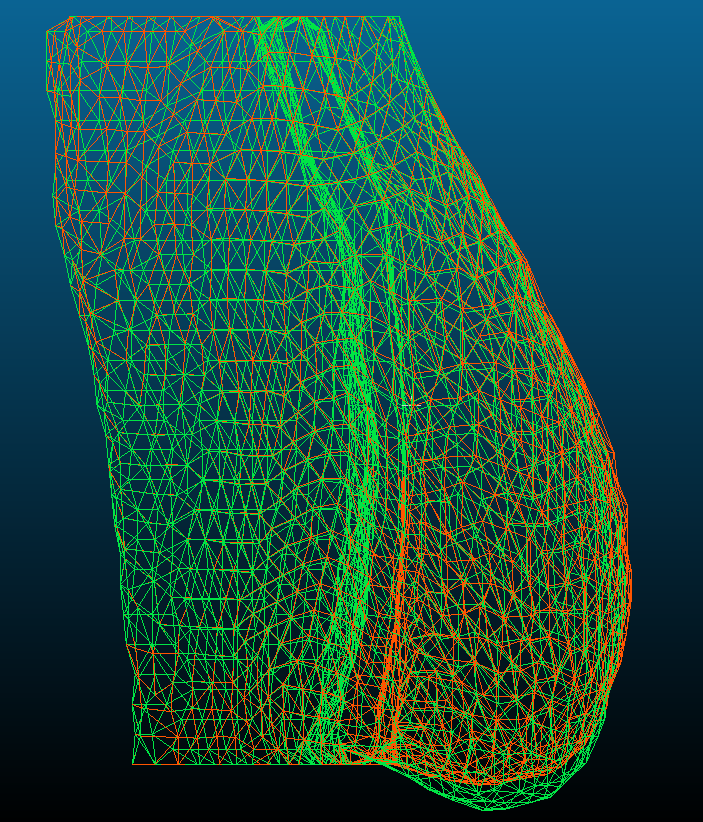
\includegraphics[width=4.5cm, height=4.5cm]{WH_example_lat} }}
    \qquad
    \subfloat[3D view]{{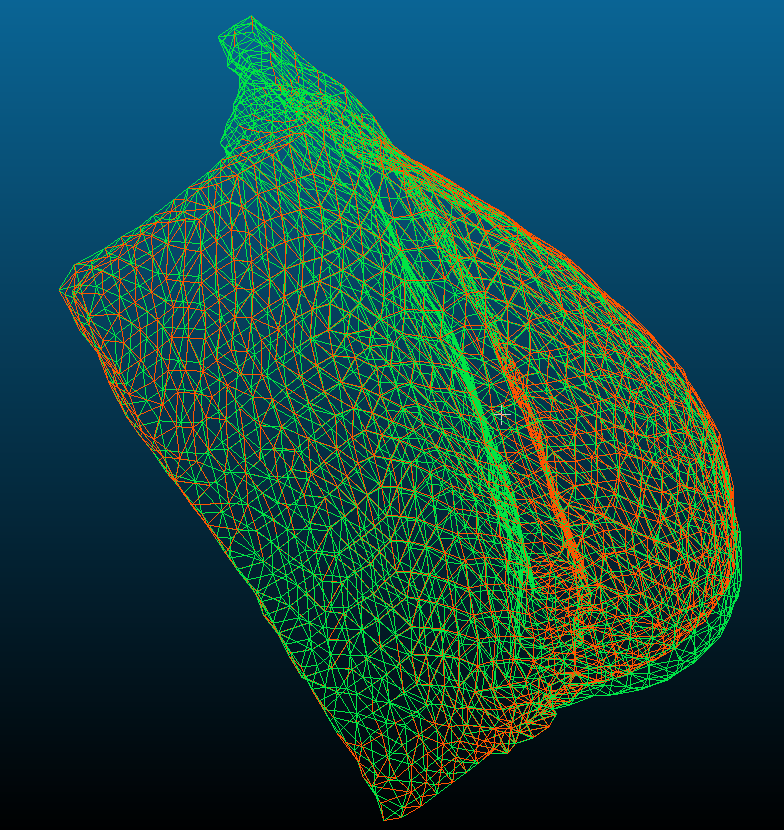
\includegraphics[width=10cm]{WH_example_3d} }}
    \caption[Wound Healing simulation]{Wound Healing simulation - comparison between the pre-surgical mesh (in green) and the pos-surgical mesh (in orange)}
    \label{fig:WHS}
\end{figure}

%\vspace{12mm}


The final dataset currently provides pre and pos-surgical models for a total of 288 possible patients based on 6 initial real patients.

Despite of the annotation for both left and right breasts, using both breasts of the same patient would lead to very similar models to the natural symmetry of the human breasts. The initial real patients used to generate all the scenarios in the semi-synthetic dataset, were choose taking into account their breast volume, being classified as small, medium or large. For each patient regardless the breast size or laterality, models were generated for all the ACR (I to IV), for all the tumor regions (1 to 4) and for all the 3 sizes (1 to 3). These combinations are illustrated in Figure \ref{fig:combinations}.

\begin{figure}[!h]
\begin{center}
    \leavevmode
    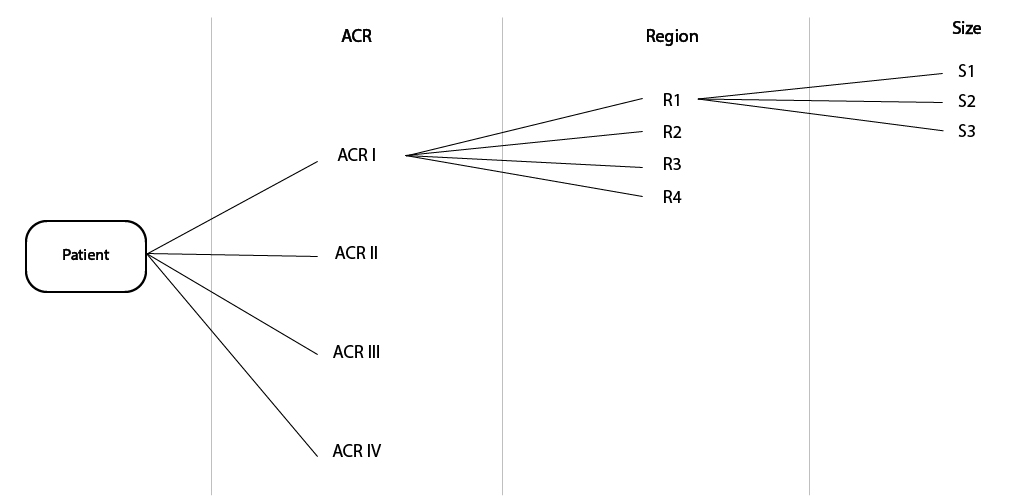
\includegraphics[width=0.8\textwidth]{combinations}
    \caption[Clinical features combinations]{Representation of possible combination of clinical features for the dataset generation}
    \label{fig:combinations}
  \end{center}
\end{figure}

All the dataset preparation steps (described previously in subsections \ref{subsec:geometry_transf}, \ref{subsection:tumor_location}, \ref{subsection:labelling} and \ref{subsection:wound_healing_simulation}) are illustrated in Figure \ref{fig:tld}.

\begin{figure}[!h]
\begin{center}
    \leavevmode
    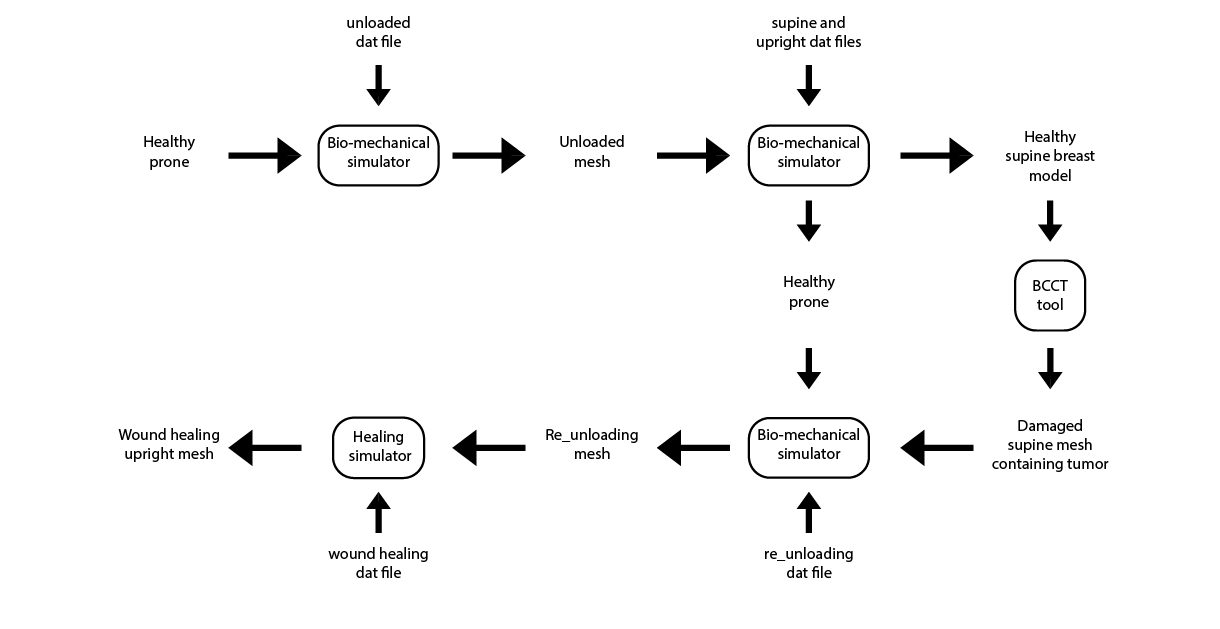
\includegraphics[width=1\textwidth]{TLD_WF-01}
    \caption[Workchart summarizing the breast's geometry transformations and wound healing simulation]{Workchart summarizing the breast's geometry transformations and wound healing simulation. The dat files are used for the Bio-mechanical simulator and the healing simulator containing the bio-mechanical and bio-chemical properties of the model's materials as well as the labelling definition.}
    \label{fig:tld}
  \end{center}
\end{figure}

\vspace{12mm}

\section{Feature Analysis and Feature Construction}

After the construction of the dataset, the data was analysed having into consideration the impact that the clinical features have on the healing simulation. Despite of the already existent and computed features, other features (like the distance between each point and the tumor's position) that were considered promising were computed and used in order to train the machine learning models.

\subsection{Feature Analysis} \label{subsec:feat_analysis}

The analysis of the clinical features was done by comparing the displacement of the corresponding points in the pre and pos-surgical models of the breast between variations of the same patient, where one of the clinical features was changing, and the others were kept the constant. The clinical features that were analysed were the tumor's size, the tumor's region and the ACR of the breast. With this study of the clinical features some conclusions were able to be drawn. The displacement of points resembles a "magnetic field" around the tumor's position and whether the tumor is located on an upper or lower region, the points of the lower region are always moved from their initial position, however, and as expected, when the tumor is located on a lower region, the displacement of the points will be larger and lead to a more profound deformation of the breast, as shown in Figure \ref{fig:region_analysis}. The impact of the tumor size can also be noticed and as expected, a bigger tumor size leads to a greater impact of the breast deformation, represented in Figure \ref{fig:size_analysis}. It is also possible to verify that the breast's density influence the deformations of the breast. A smaller ACR corresponding to a less dense breast will lead to a bigger displacement as represented in Figure \ref{fig:acr_analysis}.

\begin{figure}[!h]
\begin{center}
    \leavevmode
    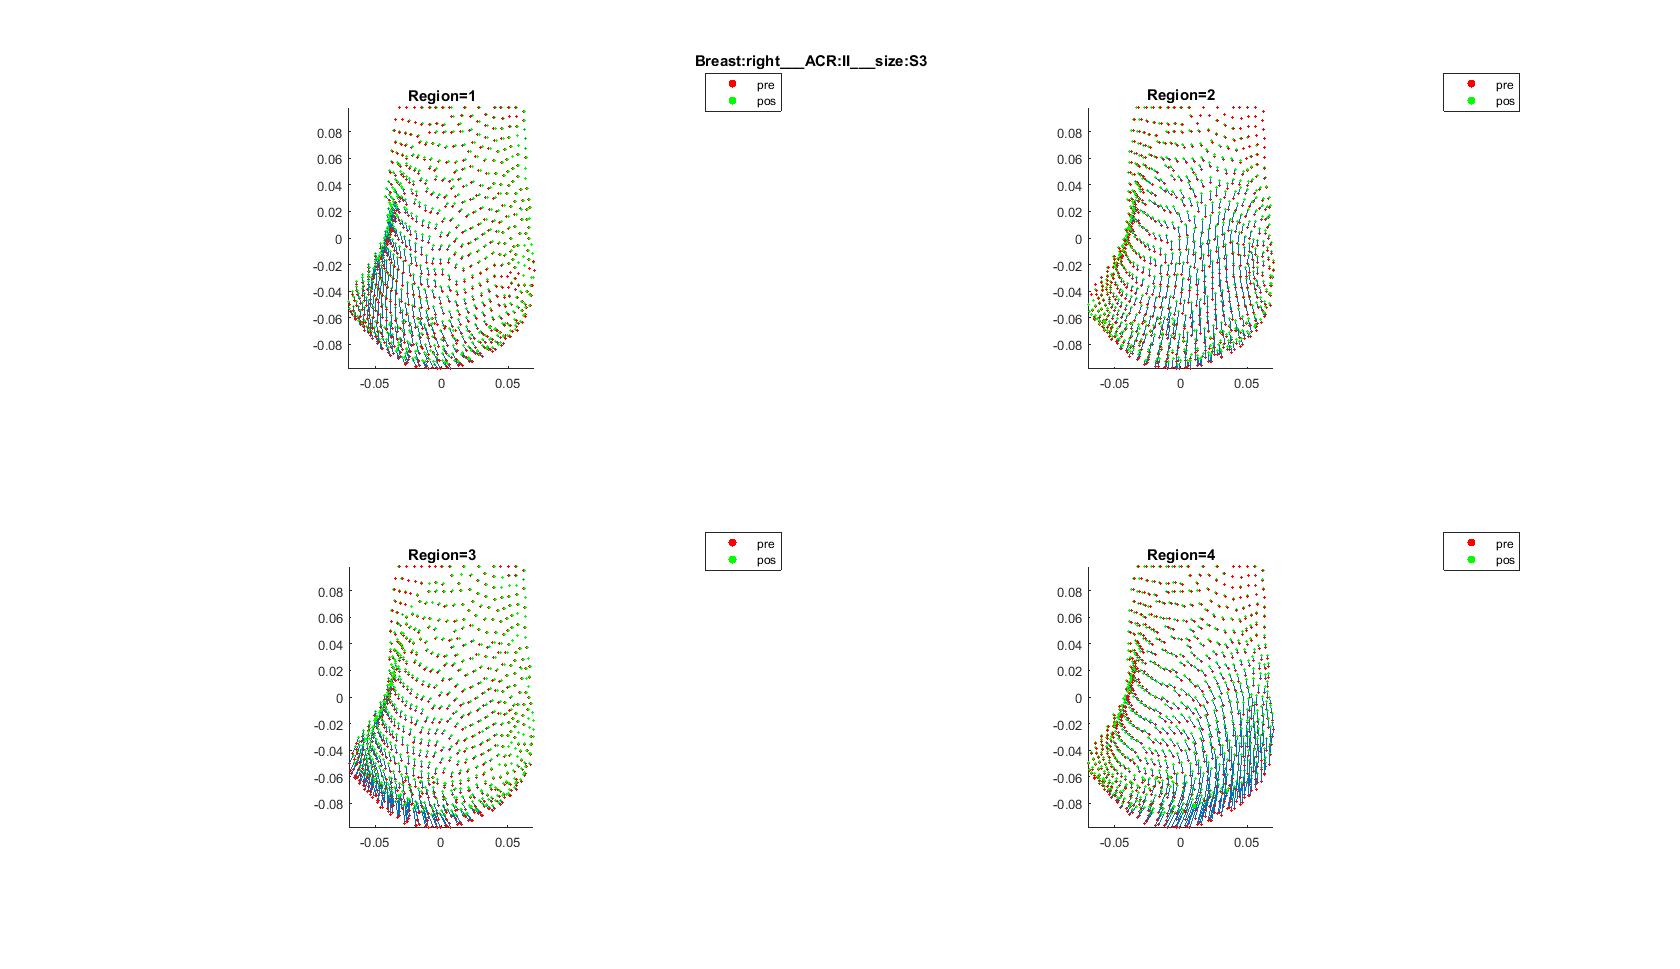
\includegraphics[width=1.2\textwidth]{region_analysis}
    \caption[Example of the impact of tumor's location (region) on the breast's deformation]{Example of the impact of tumor's location (region) on the breast's deformation}
    \label{fig:region_analysis}
  \end{center}
\end{figure}

\begin{figure}[!h]
\begin{center}
    \leavevmode
    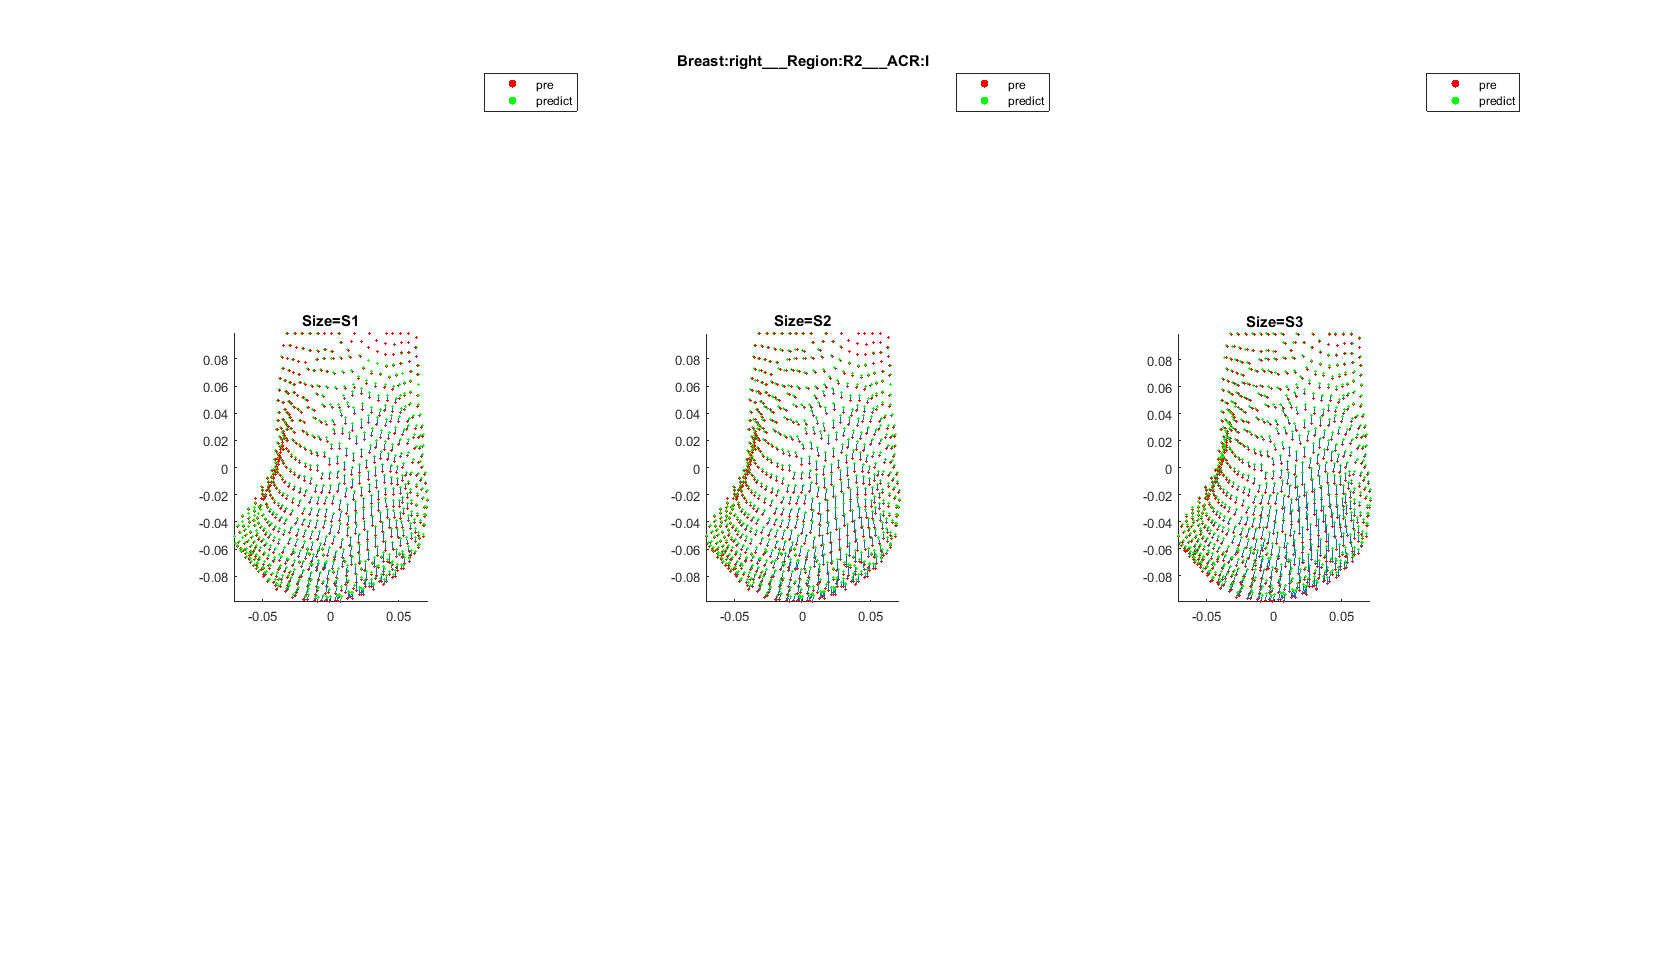
\includegraphics[width=1.2\textwidth]{size_analysis}
    \caption[Example of the impact of tumor's size on the breast's deformation]{Example of the impact of tumor's size on the breast's deformation}
    \label{fig:size_analysis}
  \end{center}
\end{figure}

\begin{figure}[!h]
\begin{center}
    \leavevmode
    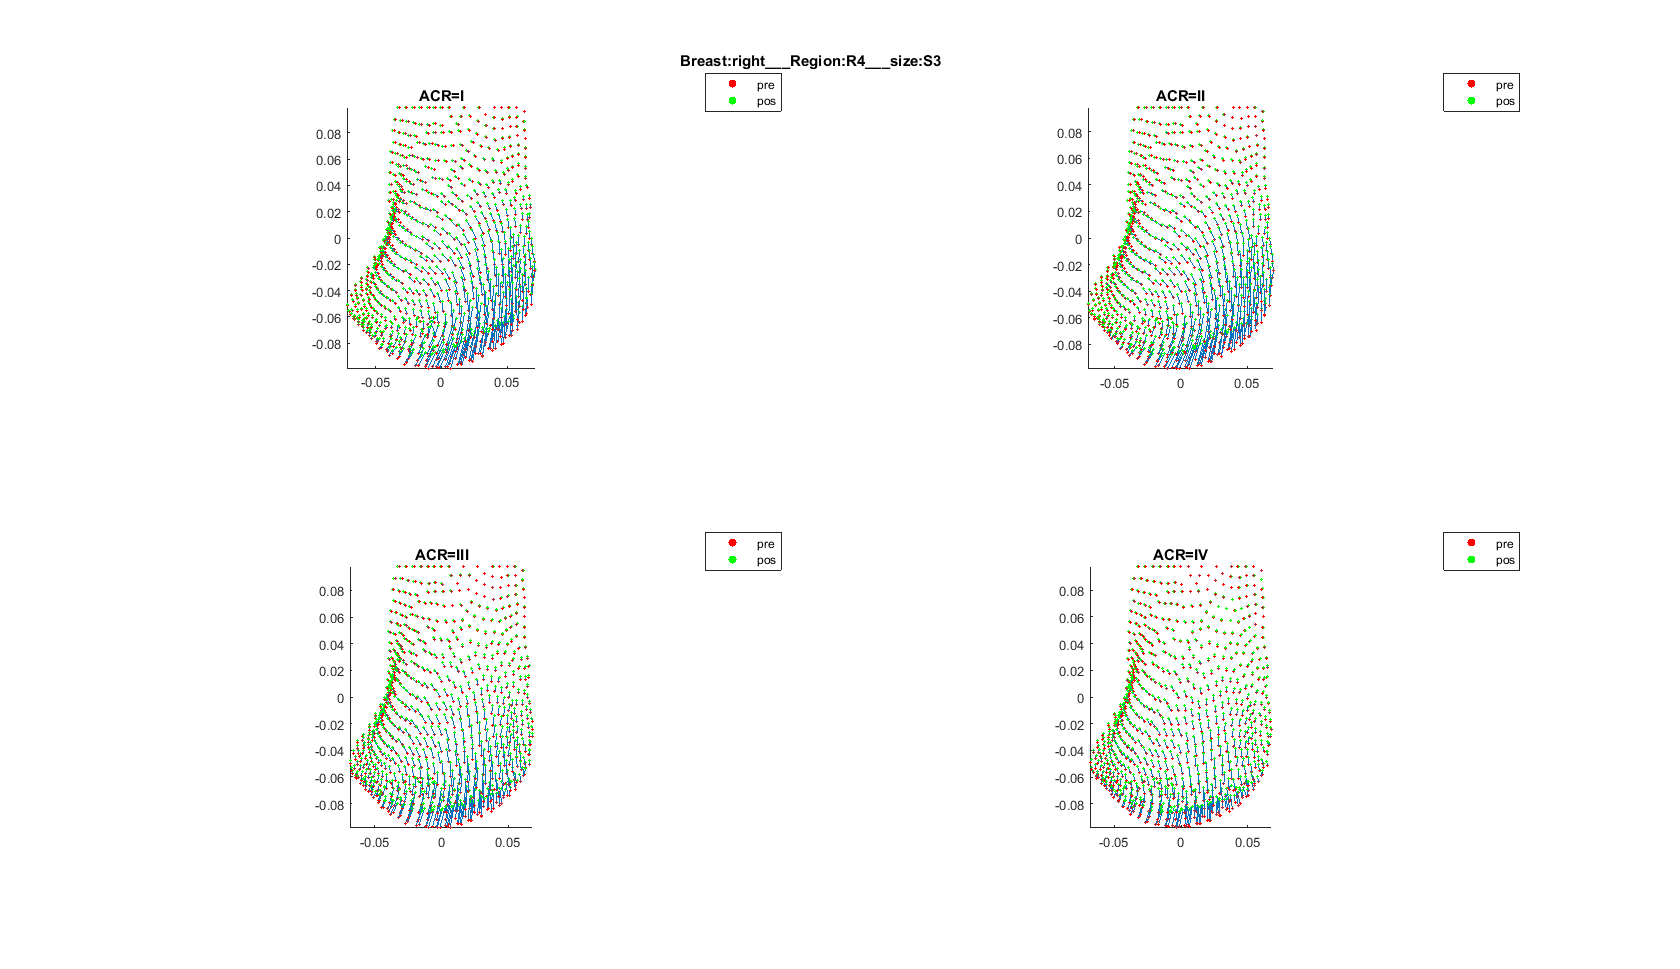
\includegraphics[width=1.2\textwidth]{acr_analysis}
    \caption[Example of the impact of breast density (ACR) on deformation]{Example of the impact of breast density (ACR) on deformation}
    \label{fig:acr_analysis}
  \end{center}
\end{figure}

Besides of these example, all the comparisons made and analyses in order to defer the impact of the clinical features on the breast deformation can be seen in appendix \ref{ap1:feat_analysis}.



\subsection{Feature Construction}

This analysis on clinical features also led to a few more conclusion about the deformation of the breast. Considering the new finding resultant from the feature analysis, some additional features were though to be helpful when trying to predict the new position of each point on the breast's point cloud. 
Despite of the findings regarding the clinical features, it was found is that the nearer surface points are to the tumour position, the more displacement they will suffer after the healing simulation. Having this in consideration, the euclidean distance and the difference for each axis, between the point itself and the tumor's center of mass, were computed and represented in both Cartesian and cylindrical coordinate. Being the cylindrical coordinates centred on the tumor's position.


\section{Model Design}

\subsection{Machine Learning Models}

As previously explained the intention of using ML (Machine Learning) Techniques is to predict the deformations caused by the BCS for the patients' breast. This prediction is carried out through the application of Regression Models which try to find a relation between the features training data, and the target values of the testing data. The target values will be the displacement of the points from the pre-surgical to the pos-surgical models of the breast.

\subsubsection{Feature Representation}

Despite of the tested scenario, the machine learning model will receive as input variables, the points of all the breasts in the training set. Each observation (as the input of the machine learning model) consists of a point from the pre-surgical model followed by several features regarding the characteristics of the breast. Initially, the training model will only have access to the points of the breast's surface, the front surface of the breast excluding the laterals, as seen in Figure \ref{fig:ML_input_pcl}. The models containing only the breast's surface that are going to be used contain an average of 629.33 point per model with a standard deviation of 106.68 points.

\begin{figure}[!h]
\centering
\begin{tabular}{cc}
\subfloat[Frontal view]{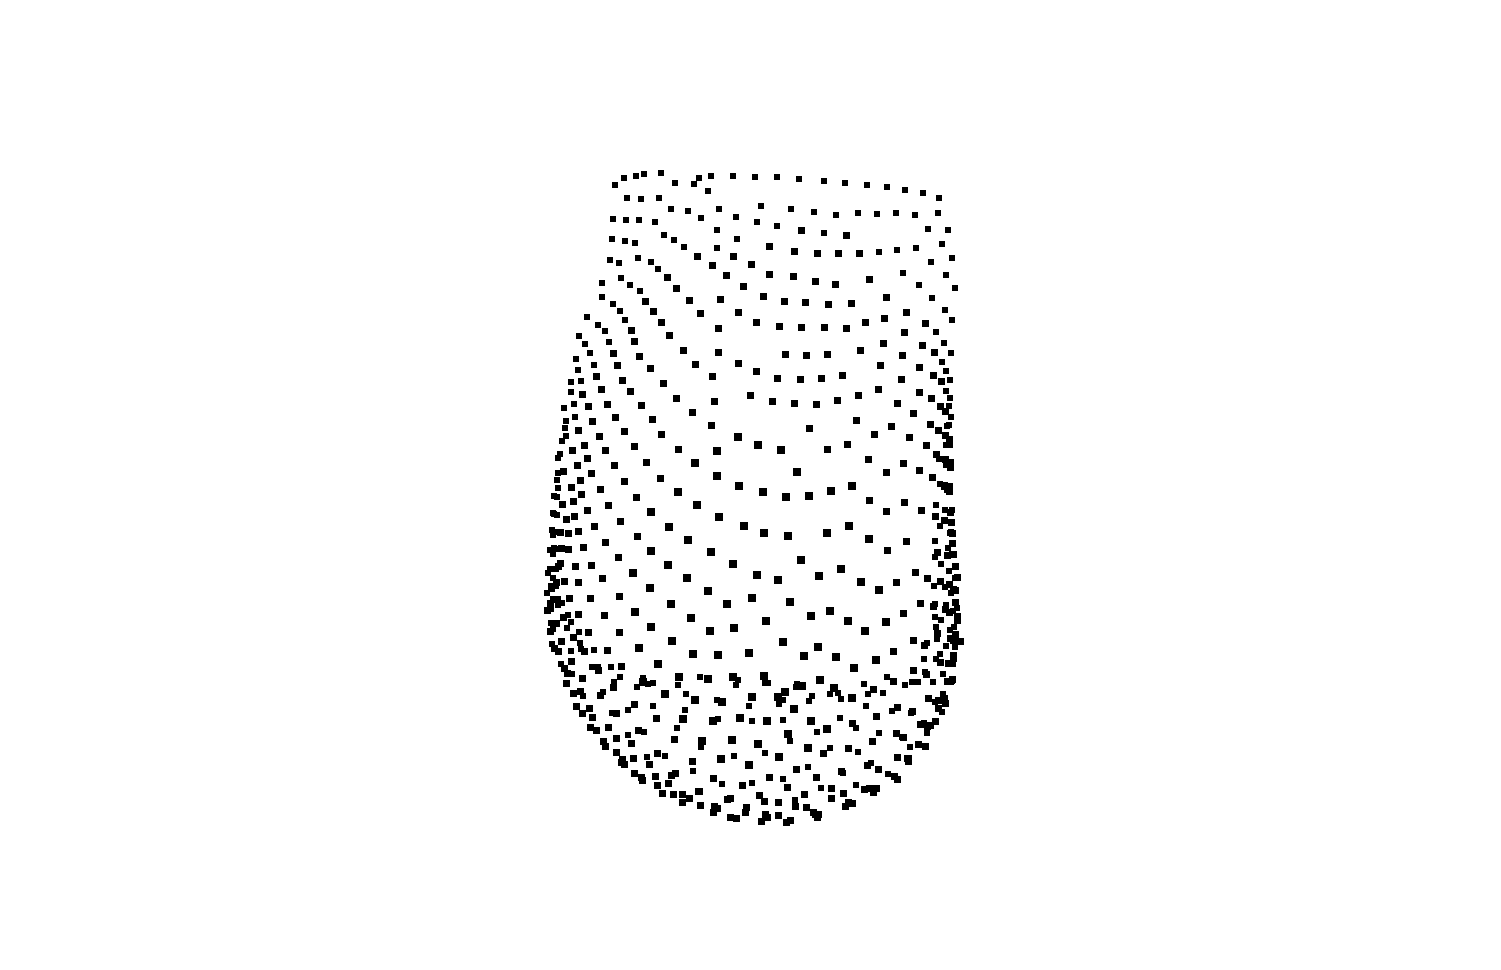
\includegraphics[width = 0.5\textwidth]{front}\label{fig:front_input}} &
\subfloat[Lateral view]{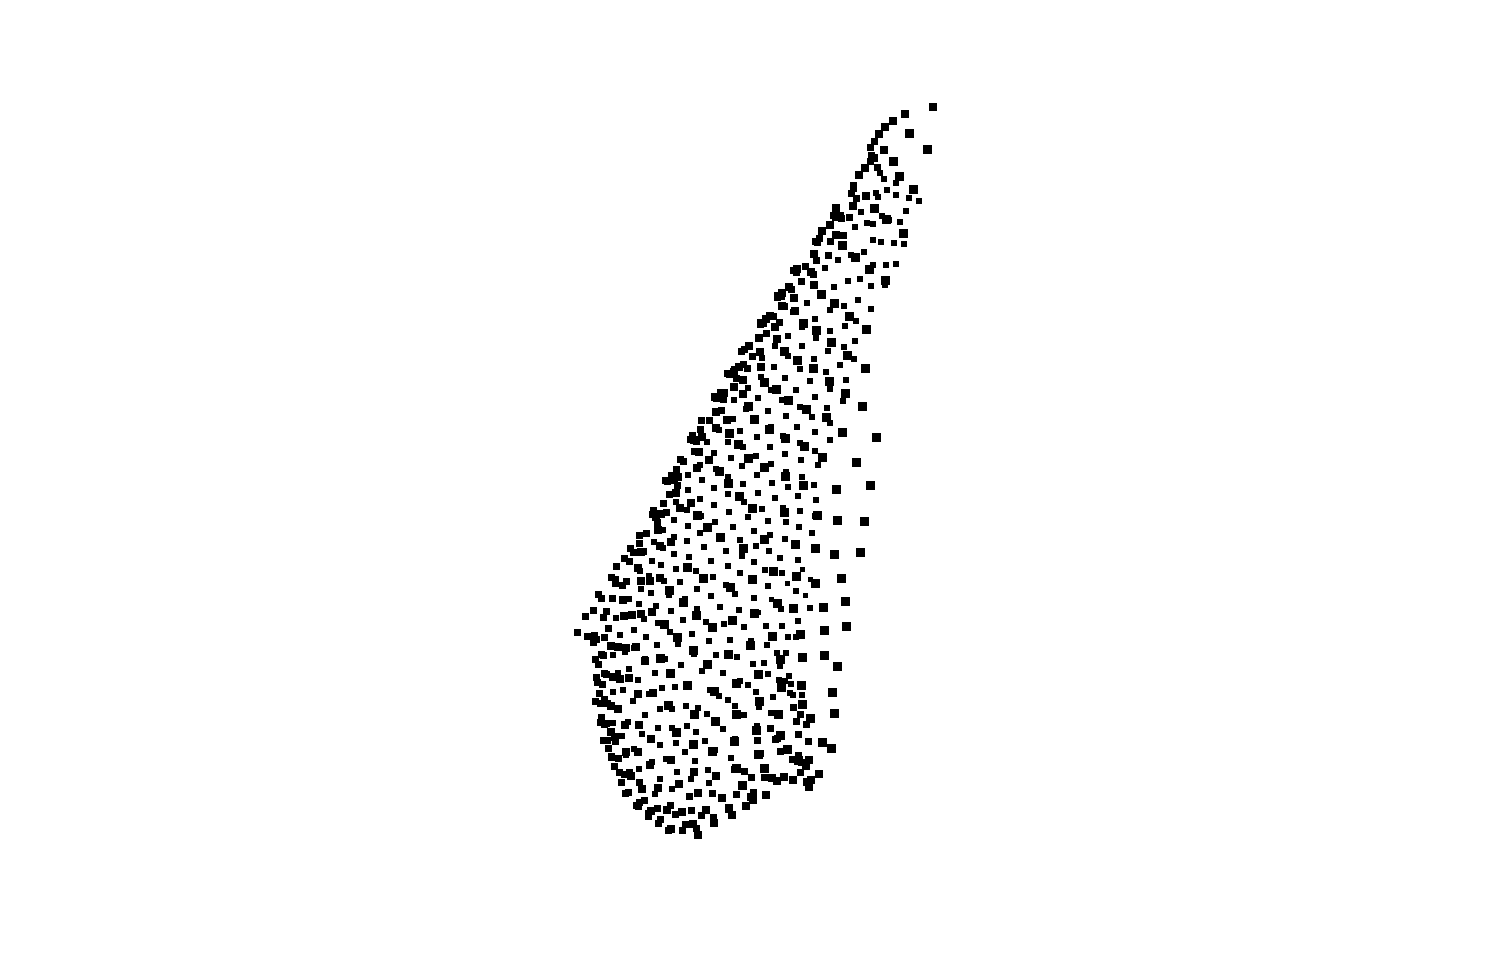
\includegraphics[width = 0.5\textwidth]{lateral}\label{fig:latearl_input}}
\end{tabular}
\caption[Example of breast point cloud to be used as ML input]{Example of breast point cloud to be used as ML input}
\label{fig:ML_input_pcl}
\end{figure}


The used features, when categorical as the laterality, the ACR of the breast, the tumor's region and tumor's size, will be represented as "dummy variables" \footnote{\url{http://imaging.mrc-cbu.cam.ac.uk/statswiki/FAQ/contint?action=AttachFile&do=get&target=int.pdf}}. Other features such as the point coordinates, breast volume, and distances will be represented as real values. 

The tumor's position defined by the breast's quadrant represents different quadrants of the breast according with the breasts laterality. For instance, while a region 4 (R4) on a left breast stands for the Lower left portion of the breast, the same region on the right breast refers to the Lower right portion. There are two possibilities in order to overcome this mismatch:
\begin{itemize}
\item Label the points according to the breast laterality, considering left and right points independent;
\item Reflect one of the breast over yOz plane or vice-versa as represented in Figure \ref{fig:reflection};
\end{itemize}

\begin{figure}[!h]
\centering
\begin{tabular}{cc}
\subfloat[left breast of a patient]{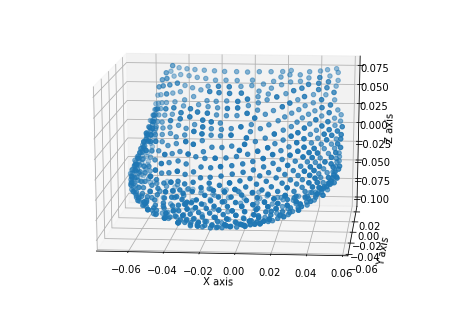
\includegraphics[width = 0.5\textwidth]{left2}\label{fig:reflection_left}} &
\subfloat[Reflection of the left breast of the patient]{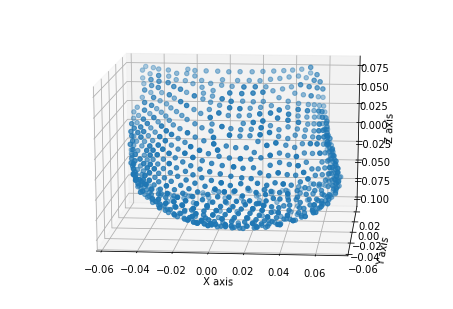
\includegraphics[width = 0.5\textwidth]{reflected2}\label{fig:reflection_reflected}}
\end{tabular}
\caption[Example of breast point cloud's reflection]{Example of breast point cloud's reflection}
\label{fig:reflection}
\end{figure}

Features like the breast laterality can be represented using categorical features or replaced by the breast's reflection. There are also features that will be represented in different ways, for instance the tumor's volume (real value of the breast's volume) and the tumor's size (categorical variable that represent the tumor as small, medium or large, regarding its size).

The Table \ref{tab:list_features} summarizes all the features that were used.

\begin{table}[!h]
%\label{tab:list_features}
\centering
\begin{tabular}{|p{16mm}|p{34mm}|p{15mm}|p{90mm}|}
\hline
\textbf{Feature}                                                     & \textbf{\begin{tabular}[c]{@{}l@{}}Feature \\ Description\end{tabular}}                                                                                                                                                                                                                                                             & \textbf{\begin{tabular}[c]{@{}l@{}}Variable\\ name\end{tabular}} & \textbf{\begin{tabular}[c]{@{}l@{}}Variable \\ Description\end{tabular}}                                                    \\ \hline \hline
\multirow{3}{*}{\begin{tabular}[c]{@{}l@{}}Point \\ coordinates\end{tabular}}                                   & \multirow{3}{*}{\begin{tabular}[c]{@{}l@{}} Point's representation \\ in a Cartesian \\ coordinate system\end{tabular}}                                                                                                                                                                                                   & x\_coord                                                            & coordinate of point in x axis                                                                                                  \\ \cline{3-4} 
                                                                     &                                                                                                                                                                                                                                                                                                                                    & y\_coord                                                            & coordinate of point in y axis                                                                                                  \\ \cline{3-4} 
                                                                     &                                                                                                                                                                                                                                                                                                                                    & z\_coord                                                            & coordinate of point in z axis                                                                                                  \\ \hline
\multirow{6}{*}{\begin{tabular}[c]{@{}l@{}} Distance's \\ projection \\ between \\ point and \\ tumor's \\ center of \\ mass\end{tabular}}                                   & \multirow{6}{*}{\begin{tabular}[c]{@{}l@{}}Distrance's projection \\ between the position \\ of the breast's point \\ and the tumor's center \\ of mass.\\ This difference can be \\ represented in a \\ Cartesian coordinate \\ system (variables \\ x\_dist, y\_dist and \\ z\_dist) or through \\ cylindrical coordinates \\ (variables theta, rho \\ and pol\_z)\end{tabular}} & x\_diff                                                             & distance's projection between the position of the point and the tumor's center of mass in a Cartesian coordinate system (x axis)          \\ \cline{3-4} 
                                                                     &                                                                                                                                                                                                                                                                                                                                    & y\_diff                                                             & distance's projection between the position of the point and the tumor's center of mass in a Cartesian coordinate system (y axis)          \\ \cline{3-4} 
                                                                     &                                                                                                                                                                                                                                                                                                                                    & z\_diff                                                             & distance's projection between the position of the point and the tumor's center of mass in a Cartesian coordinate system (z axis)          \\ \cline{3-4} 
                                                                     &                                                                                                                                                                                                                                                                                                                                    & theta                                                               & distance's projection between the position  of the point and the tumor's  center of mass in a cylindrical coordinate system (theta angle) \\ \cline{3-4} 
                                                                     &                                                                                                                                                                                                                                                                                                                                    & rho                                                                 & distance's projection between the position  of the point and the tumor's  center of mass in a cylindrical coordinate system (rho angle)   \\ \cline{3-4} 
                                                                     &                                                                                                                                                                                                                                                                                                                                    & pol\_z                                                              & distance's projection between the position  of the point and the tumor's  center of mass in a cylindrical coordinate system (z value)     \\ \hline
Distance                                                             & Euclidean distance between the point and the tumor's center                                                                                                                                                                                                                                                                & dist\_Tpt                                                           & Euclidean distance between the point and the tumor's center of mass                                                            \\ \hline
Breast's Volume                                                      & Pre-surgical breast's volume                                                                                                                                                                                                                                                                                          & b\_vol                                                              & Volume of the pre-surgical breast's model                                                                                      \\ \hline
\multirow{4}{*}{\begin{tabular}[c]{@{}l@{}}Tumor's \\ Size and \\ Volume\end{tabular}}                                & \multirow{4}{*}{\begin{tabular}[c]{@{}l@{}}Representation of the \\ tumor's volume, either \\ using the real value \\ or categorical variables\end{tabular}}                                                                                                                                                                                                                                            & t\_vol                                                              & Real value of the tumor's volume                                                                                               \\ \cline{3-4} 
                                                                     &                                                                                                                                                                                                                                                                                                                                    & t\_size\_a                                                          & Categorical variable to represent the tumor's size (small)                                                                           \\ \cline{3-4} 
                                                                     &                                                                                                                                                                                                                                                                                                                                    & t\_size\_b                                                          & Categorical variable to represent the tumor's size (medium)                                                                          \\ \cline{3-4} 
                                                                     &                                                                                                                                                                                                                                                                                                                                    & t\_size\_c                                                          & Categorical variable to represent the tumor's size (large)                                                                           \\ \hline
\multirow{2}{*}{\begin{tabular}[c]{@{}l@{}}Breast's \\ Laterality\end{tabular}}                                                               & \multirow{2}{*}{\begin{tabular}[c]{@{}l@{}}Representation of the \\ breast's laterality \\ (left or right breast)\end{tabular}}                                                                                                                                                                                                                                            & lat\_a                                                              & Categorical variable to represent the breast's laterality (Right Breast)                                                             \\ \cline{3-4} 
                                                                     &                                                                                                                                                                                                                                                                                                                                    & lat\_b                                                              & Categorical variable to represent the breast's laterality (Left Breast)                                                              \\ \hline
\multirow{4}{*}{\begin{tabular}[c]{@{}l@{}}Breast's \\ Density \\ (ACR)\end{tabular}}                                                           & \multirow{4}{*}{\begin{tabular}[c]{@{}l@{}}Representation of the \\ breast's density \\ using ACR\end{tabular}}                                                                                                                                                       & acr\_a                                                              & Categorical variable to represent the breast's density (ACR I)                                                                       \\ \cline{3-4} 
                                                                     &                                                                                                                                                                                                                                                                                                                                    & acr\_b                                                              & Categorical variable to represent the breast's density (ACR II)                                                                      \\ \cline{3-4} 
                                                                     &                                                                                                                                                                                                                                                                                                                                    & acr\_c                                                              & Categorical variable to represent the breast's density (ACR III)                                                                     \\ \cline{3-4} 
                                                                     &                                                                                                                                                                                                                                                                                                                                    & acr\_d                                                              & Categorical variable to represent the breast's density (ACR IV)                                                                      \\ \hline
\multirow{4}{*}{\begin{tabular}[c]{@{}l@{}}Tumor's \\ Location \\ (Region)\end{tabular}}                                                        & \multirow{4}{*}{\begin{tabular}[c]{@{}l@{}}Representation of the \\ tumor's location \\ regarding the breast's \\ quadrant\end{tabular}}                                                                                                                                                                                                                                            & reg\_a                                                              & Categorical variable to represent the tumor's located in R1                                                                          \\ \cline{3-4} 
                                                                     &                                                                                                                                                                                                                                                                                                                                    & reg\_b                                                              & Categorical variable to represent the tumor's located in R2                                                                          \\ \cline{3-4} 
                                                                     &                                                                                                                                                                                                                                                                                                                                    & reg\_c                                                              & Categorical variable to represent the tumor's located in R3                                                                          \\ \cline{3-4} 
                                                                     &                                                                                                                                                                                                                                                                                                                                    & reg\_d                                                              & Categorical variable to represent the tumor's located in R4                                                                          \\ \hline
\end{tabular}
\caption{List of Features}
\label{tab:list_features}
\end{table}

\subsubsection{Labels} \label{subsec:labels}

In order to obtain the shape of the breast after the BCS, the trained machine learning models predict the displacement of the points between the pre-surgical and pos-surgical models of the breast in each axis. This displacement is calculated by computing the difference in each axis between the pos-surgical point of the 3D model and the correspondent point in the pre-surgical 3D model. Through the feature analysis described in subsection \ref{subsec:feat_analysis}, it is evident that the axis where the points suffer a larger displacement is the \textit{z} axis.

\vspace{12mm}

Having the dataset ready with both the features and labels computed, the dataset was split into training and testing sets. This division was done in two different ways:
\begin{itemize}
\item Splitting the dataset by applying a Leave-one-out (LOO) methodology. The dataset is divided into 6 sets of data (one per each initial real patient, containing 48 cases each), and using alternately each one of the sets as test set and the remaining 5 sets as training set;
\item Randomly split the 288 cases of the complete dataset using 1/6 of the cases as testing set and the remaining cases (5/6) as training set.
\end{itemize}

Regarding the validation set, the models use 10-fold cross validation. As expected and as can be seen in chapter \ref{chap:results}, randomly splitting the data leads to much better although misleading results than the other approach for the splitting of the dataset into training and testing sets. This is justified by the similarity of the breast within the training and the testing set, since both of them are simulations of the same initial patient despite of the different clinical features. The use of this biased testing set allowed the representation of a best case scenario for the prediction of the breast's deformation.

\subsubsection{Machine Learning Algorithms} \label{subsec:implementation}

In order to train the machine learning models that will be used to predict the displacement of the pre-surgical model to the pos-surgical, the following machine learning algorithms were used in order to solve this regression problem. 

\begin{itemize}
\item Multilayer Perceptron (MLP)

MLP, also known as feedforward neural networks (FFNN) is a type of Artificial Neural Networks widely used when targetting clinical medical issues \cite{Finne2000}. They consist of a set of nodes connected by edges that simulate the behaviour of neurons of the human brain. \cite{Nygren2016}

The node is responsible to compute the weighted sum of the inputs  $ z = \sum_{j=1}^{m} w_j x_j $ and to apply an activation function $ y = \varphi (z+b) $, where $x_j$ is the input for input link $j$ , $w_j$ the weight for the same input, $y$ the output of the neuron, $b$ the optimal bias parameters added to the input and $\varphi$ is an activation function.

An example of a MLP is represented in Figure \ref{fig:NN} consisting of multiple layers of fully connected neurons. The represented layers differ in three types:
\begin{itemize}
\item Input layers - only transport all the inputs to the next layer; 
\item Hidden layers - adjust the weighed sum of the inputs, compute the activation function and output the values to the next layer;
\item Output layers - perform the same computations that hidden layers do and output the values as the network's result.
\end{itemize}

\begin{figure}[!h]
\begin{center}
    \leavevmode
    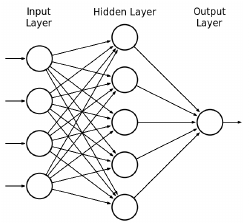
\includegraphics[width=0.5\textwidth]{NN}
    \caption[Representation of a MLP]{Representation of a MLP \cite{Ortiz2016}}
    \label{fig:NN}
  \end{center}
\end{figure}

The number of neurons highly depends on the amount and properties of the training data, as well as the number of hidden layers. And the Learning rate impacts the step used to adjust the inputs' weight.

\item Random Forest (RF)

The Random Forest (RF) algorithm is based on using multiple decisions trees, mitigating the negative aspects of decision trees by ignoring some of the input properties and increasing the performance of the algorithm.
Each decision tree on the RF system, only consider a random subset of the input data, and consider a limited number of features smaller than the number of total features. The output of the several decision trees is then averaged and used as output of the RF \cite{Nygren2016}.

The splitting criteria for regression problems in RF algorithms to divide the root or leaf into more leafs is calculate through $ RSS = \sum_{LEFT} (Y_i - Y_{L}^{*})^{2} + \sum_{RIGHT} (Y_i - Y_{R}^{*})^{2}$, where $RSS$ stands for Residual sum of the squares, $Y_i$ stands for the current node and $Y_L^{*}$ and $Y_R^{*}$ stands for the mean value of \textit{y} for both the left and right nodes, respectively \cite{Cutler2013}.

Figure \ref{fig:RF} presents an example of a decision tree regression result.

\begin{figure}[!h]
\begin{center}
    \leavevmode
    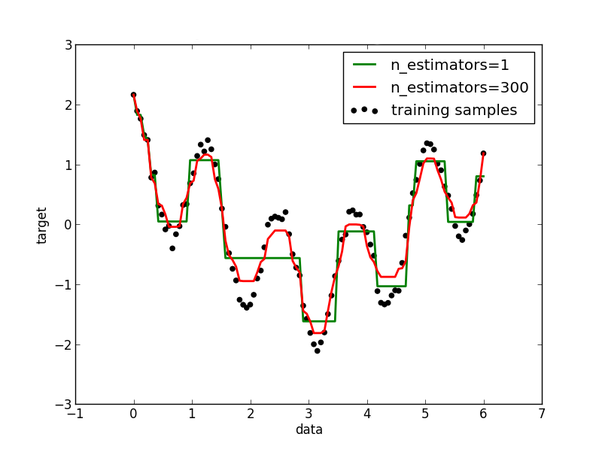
\includegraphics[width=0.7\textwidth]{RF}
    \caption[Example of a RF result]{Example of a RF result. Comparison of results of a RF with only a decision tree (green) and a RF with 300 decision trees (red). The scatter point represent the data used to train the RF. \protect\footnotemark}
    \label{fig:RF}
  \end{center}
\end{figure}
\footnotetext{\url{https://www.quora.com/How-does-random-forest-work-for-regression-1}}

This type of algorithm has as great advantage not requiring a prior feature section, and despite of being promising, it is only capable of predicting the regression of a variable. In this case, in order to predict the total displacement of the point between models, three individual training models are required, one for each Cartesian axis.

\item Multioutput Regression (MOR)

Multioutput regression also known as multi-variate or multi-target regression, has been used on multiple applications across several fields of study \cite{Borchani}. This ML approach allows the prediction of several output variables for each entry of the model. \footnote{\label{mor} \url{http://scikit-learn.org/stable/modules/multiclass.html\#multiclass}} Other advantage of this type of approach is that the produced models are, generally, simpler and more computational efficient.

One of the several multioutput regression method consists on the adaptation of other ML algorithms such as RF in order to allow them to predict several output variables. This type of multioutput regressors requires the identification of the dependencies among the target variables. When compared to regular RF, multi-target regression trees usually require a smaller number of trees for all the variables, and allow a more informed understanding of the dependencies among the several target variables of the model \cite{Borchani}.


\end{itemize}


\subsubsection{Implementation}

As already stated, the presented algorithms were implemented aiming to predict the displacement between the pre-surgical and the pos-surgical models. The displacement for \textit{x} axis, \textit{y} axis and \textit{z} axis are respectively represented as \textit{$\partial$x}, \textit{$\partial$y} and \textit{$\partial$z}.

The 3 previously described machine learning algorithms were implemented using 10 fold cross validation in order to automatically tune each algorithm parameters leading the algorithm to achieve the minimum root mean squared error of the model. The 3 algorithms were used to train both of the splits of the dataset (LOO and the random split using 1/6 of the data as the test set).

A short feature selection was done to understand which features should be used as well as their representations. The feature selection was done recurring to recursive feature elimination \footnote{\url{https://topepo.github.io/caret/recursive-feature-elimination.html}}, and then a trial was done using MLP. Regarding the training of RF and MOR, this study was not necessary since both algorithms support a built-in feature selection method that measures the feature's importance \footnote{\url{https://topepo.github.io/caret/feature-selection-overview.html}}. The last two algorithms led to the training of random forest models for each axis (\textit{x}, \textit{y} and \textit{z} axis); and the training of multi output regressor models, considering the \textit{$\partial$z}, \textit{$\partial$y}, \textit{$\partial$x} as labels; \textit{$\partial$y} and \textit{$\partial$x} as labels; and \textit{$\partial$x} and \textit{$\partial$y} as labels.

In order to implement the random forests and multi-layer perceptron algorithms a R package named caret \footnote{\label{caret} \url{https://cran.r-project.org/web/packages/caret/caret.pdf}} was used. Multi-output regressor was implemented with a R package called randomForestSRC package \footnote{\label{rfsrc} \url{https://cran.r-project.org/web/packages/randomForestSRC/randomForestSRC.pdf}}.

\subsection{Naive Model} \label{sub_sec:naive_method_explanation}

In order to understand the impact of ML techniques to predict the deformation, a naive method was created to generate the shape of the breast using common sense and conclusion arising from the feature analysis presented in section \ref{subsec:feat_analysis}.

Two alternatives for the naive method were developed, where the displacement between the pre-surgical and pos-surgical models of the breast were computed as follows:
\begin{enumerate}
\item The first alternative consisted on calculating the average displacement of the points on each geometric quadrant of the breast. The average displacement of each quadrant is calculated based on the mean displacement of the points on the same quadrant in similar breasts. These similar breast concerns all the breasts on the dataset, that were generated from a different initial patient, with the same breast properties: breast's laterality and density and the same tumor's properties.

For instance, if the breast that is under the naive method has the tumor located in region 2, the average displacement for the correspondent quadrant will be calculated based on the other patients with the tumor on the same region, the same tumor's size and the same breast's laterality and density. For the regions were the tumor is not located, the average displacement will be calculated based on the breasts of the dataset, that do not have the tumor located on that region and with the same breast's properties and tumor's size. Therefore, the quadrants are defined based on the geometric center of the breast.

In spite of calculating an average displacement for the all quadrants of the breast, only a portion of that displacement is applied to the pre-surgical model. Each quadrant was divided into 3 stacks across the z axis, and a portion or the total displacement was applied based on how much the points on that region would normally move. The stack division is done equally, however the portion of the applied displacement on the \textit{x}, \textit{y} and \textit{z} axis differs according to the quadrants (lower or upper quadrant).

\item  The second approach of the naive method, is divided into two steps. In the first step, and similar with what happens on the first approach, the breast is divided into quadrants, however considering the nipple's position but not the geometric center of the breast. In the second step, and taking into consideration all breasts in the dataset, the average displacement of points is calculated for each quadrant of the breast. When considering the quadrant where the tumor is located, the points below the tumor are updated by subtracting their height from the mean displacement previously calculated; When considering the not affected quadrants (without the tumor located on them), the points' position is updated. Calculating the ratio between the average displacement of the non-affected quadrants and the distance from the point to the tumor's center of mass, will give a value that, when subtracted from the point's previous position will result on the new position of the point. The computed displacements are also multiplied by the breasts' ACR using a factor of 1.2, due to the relation between the breast's ACR and the breast's deformation.

\end{enumerate}

\section{Results Validation}

Despite of the use of cross validation and the parameter tuning used on the implementation of the machine learning models that tried to decrease the root mean squared error between the predicted data and the given labels, the obtained results were evaluated using some evaluation metrics. As previously described, the given machine learning models had as goal to predict the displacement of each point in the breast's 3D model in one or more axis. Summing the predicted values to the correspondent point of the pre-surgical breast's model, ideally would produce the pos-surgical model of the breast.

\subsection{Evaluation Metrics}

There were considered two types of evaluation metrics:
\begin{itemize}
\item Visual metrics;

The visual metrics consists of visual comparison between pre-surgical, pos-surgical and predicted models of the breast. This evaluation allows to easily gather some conclusion regarding the models performance.

\item Distance metrics.

The distance metrics allows to obtain a more accurate perception of the model's performance.
\end{itemize}

\subsubsection{Distance metrics}

The distances computed for evaluating the models consider both local and global distances: while, the local distance, compare the models point by point, the global distances is measured in both directions comparing each point of a model to another breast's model and a breast's model to a point of another model. Regarding the local metric, the distances to be measured are the one between the predicted model and the pos-surgical model (\textit{predicted to pos}); the distance between the pre-surgical to the pos-surgical models (\textit{pre to pos}); and the distance between the predicted model and the pre-surgical model (\textit{predicted to pre}). Regarding the global metric, the same distances will be measures, however in both directions: \textit{predicted to pos}; \textit{pos to predicted}; \textit{pre to pos}; \textit{pos to pre}; \textit{predicted to pre}; and \textit{pre to predicted}. 

On either case the following values are computed:
\begin{itemize}
\item Mean of Euclidean distance;
\item Standard Deviation of the Euclidean distance;
\item Hausdorff distance (maximum of the euclidean distances).
\end{itemize}

These values are calculated considering the 3 coordinates of each point (3D), or only the point's projection in one of the Cartesian coordinate system axis(1D).


\section{Summary}

The present chapter, described the complete process that was followed in order to predict the deformation caused by BCS. Initially the dataset preparation was described, and some additional information was given, in order to understand its construction. Then a analysis of the clinical features was also detailed and results presented in the chapter. Thereafter the models used in order to predict the breast deformations were explained. Regarding the introduced machine learning techniques, a short background of the regression models was provided and all the relevant information about their implementation and application is outlined. At last, the evaluation metrics were also described.

All the results and further conclusion arising from the detailed methodology are explored in chapter \ref{chap:results}. 



